% ============================================================================
%  IMU Calibration and Attitude Estimation for a Four-Wheel Skid-Steer Robot
%  Documentation of IMU_CALIBRATE.cpp (guided test), attitude.h (attitude
%  filter), MPU6050_Custom (driver) and the IMU path in main.cpp.
%  Compile with pdflatex, twice (table of contents and references).
% ============================================================================
\documentclass[11pt,a4paper]{report}

\usepackage[utf8]{inputenc}
\usepackage[T1]{fontenc}
\usepackage{lmodern}
\usepackage[margin=2.5cm]{geometry}
\usepackage{amsmath,amssymb}
\usepackage{graphicx}
\usepackage{float}
\usepackage{booktabs}
\usepackage{array}
\usepackage{longtable}
\usepackage{xcolor}
\usepackage{listings}
\usepackage{enumitem}
\usepackage{fancyhdr}
\usepackage{caption}
\usepackage{tikz}
\usetikzlibrary{arrows.meta,positioning,shapes.geometric,calc}
\usepackage{pgfplots}
\pgfplotsset{compat=1.16}
\usepackage[hidelinks]{hyperref}

\setlength{\parindent}{0pt}
\setlength{\parskip}{6pt}
\setlength{\headheight}{14pt}
\pagestyle{fancy}
\fancyhf{}
\fancyhead[L]{IMU Calibration and Attitude Estimation}
\fancyhead[R]{\small\leftmark}
\fancyfoot[C]{\thepage}
\renewcommand{\headrulewidth}{0.4pt}

\definecolor{codegray}{gray}{0.95}
\definecolor{warnred}{RGB}{160,30,30}
\lstset{
  basicstyle=\ttfamily\footnotesize,
  backgroundcolor=\color{codegray},
  breaklines=true,
  frame=single,
  columns=fullflexible,
  keepspaces=true,
  showstringspaces=false,
  tabsize=2
}

\newcommand{\code}[1]{\texttt{#1}}
\newcommand{\todo}[1]{\textcolor{warnred}{\textbf{[TODO: #1]}}}
\newcommand{\dps}{^{\circ}\!/\mathrm{s}}
\newcommand{\mps}{\,\mathrm{m/s^2}}

\newcommand{\photo}[2]{%
  \begin{figure}[H]\centering
  \fbox{\parbox[c][5.5cm][c]{0.85\textwidth}{\centering\Large PHOTO PLACEHOLDER\\[4pt]\normalsize #1}}
  \caption{#1}\label{#2}
  \end{figure}}

\newcommand{\plotph}[2]{%
  \begin{figure}[H]\centering
  \fbox{\parbox[c][6cm][c]{0.85\textwidth}{\centering\Large SCREENSHOT / PLOT PLACEHOLDER\\[4pt]\normalsize #1}}
  \caption{#1}\label{#2}
  \end{figure}}

\newcommand{\warnbox}[1]{%
  \par\noindent\fcolorbox{warnred}{white}{\parbox{0.96\textwidth}{\textbf{\textcolor{warnred}{Warning.}} #1}}\par}

\newcommand{\verifybox}[1]{%
  \par\noindent\fcolorbox{blue!50!black}{blue!5}{\parbox{0.96\textwidth}{\textbf{Verification note.} #1}}\par}

\title{\textbf{IMU Calibration and Attitude Estimation\\for a Four-Wheel Skid-Steer Robot}\\[6pt]
\large Guided Test Firmware (\code{IMU\_CALIBRATE.cpp}), Attitude Filter (\code{attitude.h}),\\Sensor Driver, and Integration into the Odometry Chain}
\author{[Author name]\\[0pt] {[Institution / Department]}}
\date{2026-10-17}

\begin{document}
\maketitle

\begin{abstract}
The heading that the robot publishes in \code{/odometry/filtered} is the time integral of one gyroscope axis, so every error of that gyroscope appears directly in the pose that Nav2 and the SLAM stack receive. This report documents how the inertial sensor, an MPU6050 on I$^2$C, is characterised, corrected and used. It covers four parts: the guided test firmware \code{IMU\_CALIBRATE.cpp}, which in four stages (still, one full turn, nose up, left side up) measures offsets, noise, gyro scale and sign conventions; the sensor driver \code{MPU6050\_Custom}, which applies stored static offsets and a boot-time gyro bias; the roll and pitch complementary filter \code{attitude.h}, with its accelerometer gain correction, gravity compensation and ramp detector; and the way \code{main.cpp} combines these with a zero-velocity update, a dead-band and a four-state extended Kalman filter. The report gives the error models and the equations behind each step, the exact operating procedure with acceptance criteria and formulas for updating the stored constants, a validation record from hand-turn tests, Python replicas of the filter and of the EKF heading path that check specific claims, a troubleshooting guide, and a list of limitations found while reading the code. Result tables and photo slots are left blank for the commissioning data.
\end{abstract}

\tableofcontents
\listoffigures
\listoftables

% ============================================================================
\chapter{Introduction}
% ============================================================================

\section{Motivation}
A wheeled robot that maps and navigates autonomously needs a pose estimate whose errors stay small between the moments when the lidar corrects it. On a skid-steer chassis the wheels slip sideways during every turn, so wheel odometry under-reads rotation by an amount that depends on the floor. The gyroscope does not have that problem, which is why the firmware takes yaw from the gyro alone. The price is that the gyro's own errors, a scale error, a residual bias and noise, are no longer averaged against anything else. A scale error of 0.4\,\% is 1.5$^\circ$ per full turn; a residual bias of 0.001\,rad/s is 3.4$^\circ$ per minute of driving. Both are small, and both are worth measuring rather than assuming.

The same sensor provides roll and pitch, used to remove gravity from the forward acceleration that feeds the velocity estimate and to flag when the robot is on a ramp.

\section{Scope}
This document covers:
\begin{itemize}[noitemsep]
  \item the guided test firmware \code{IMU\_CALIBRATE.cpp} (its header comment calls it \code{imu\_guided\_test.cpp}, see Chapter~\ref{ch:limits});
  \item the attitude filter \code{attitude.h};
  \item the driver \code{MPU6050\_Custom.h/.cpp};
  \item the IMU, ZUPT, dead-band and EKF heading path in \code{main.cpp}.
\end{itemize}
It does not cover the lidar, SLAM, or the wheel speed loops (see the companion report on \code{PID\_TEST.cpp} and \code{motor\_calibrate.py}). The robot has no magnetometer, so absolute heading is not available and heading is always relative to the pose at power-up.

\section{Conventions and notation}
Frames and signs follow ROS REP-103: the body frame is \emph{forward--left--up} (FLU), right-handed, with $x$ forward, $y$ to the left and $z$ up. Angles are in radians internally and degrees in console output. Table~\ref{tab:notation} lists the symbols.

\begin{table}[H]
\centering
\caption{Symbols used in this report.}\label{tab:notation}
\small
\begin{tabular}{@{}llp{8.2cm}@{}}
\toprule
Symbol & Unit & Meaning\\
\midrule
$a_x,a_y,a_z$ & m/s$^2$ & Specific force in the body frame (accelerometer output)\\
$p,q,r$ (or $g_x,g_y,g_z$) & rad/s & Body angular rates about $x$, $y$, $z$\\
$\phi$ & rad & Roll, positive when the left side is up\\
$\theta$ & rad & Pitch, positive when the nose is down\\
$\psi$ & rad & Yaw, positive counter-clockwise seen from above\\
$G$ & m/s$^2$ & Standard gravity, 9.80665\\
$k$ (\code{k\_}) & -- & Accelerometer gain correction, $G/\lVert\mathbf a\rVert$ at calibration\\
$b$, $\hat b$ & rad/s & True and estimated gyro bias\\
$s$ & -- & Gyro scale error: measured rate $=(1+s)\times$ true rate\\
$\tau$ & s & Complementary-filter time constant, 1.0\\
$\alpha$ & -- & Gyro weight per step, $\tau/(\tau+\Delta t)$\\
$\Delta t$ & s & Sample period: 0.05 in \code{main.cpp}, 0.02 in the test\\
$\lambda$ & -- & ZUPT gain per sample, 0.02\\
$N_{\mathrm{ARW}}$ & rad/$\sqrt{\mathrm s}$ & Angle random walk coefficient\\
\bottomrule
\end{tabular}
\end{table}

\section{Precautions}
\warnbox{\code{IMU\_CALIBRATE.cpp} contains no motor code and never configures the motor driver pins, so nothing is driven. Even so, an unconfigured driver input can float, and some drivers respond to that. Disconnect the motor battery, or put the robot on a stand with the wheels free, before flashing. The spin stage is done by hand: keep the robot flat on the surface, and keep the USB cable slack so that it does not drag on the robot or pull the board.}

\photo{Robot on a level table with the motor battery disconnected, ready for the IMU test.}{fig:setup}

% ============================================================================
\chapter{System Description}
% ============================================================================

\section{Hardware}
The inertial sensor is an MPU6050 (3-axis gyroscope and 3-axis accelerometer) read over I$^2$C at address 0x68 through the \code{Wire} library on the pins \code{I2C\_SDA} and \code{I2C\_SCL} from \code{pins.h}. It shares the bus with the TCS34725 colour sensor. Table~\ref{tab:hw} lists the facts the report relies on; the rest is to be filled in.

\begin{table}[H]
\centering
\caption{Hardware summary. Items marked \todo{} are for the builder to complete.}\label{tab:hw}
\small
\begin{tabular}{@{}ll@{}}
\toprule
Item & Value\\
\midrule
Microcontroller & ESP32-S3 (Arduino framework, PlatformIO)\\
IMU & MPU6050, I$^2$C 0x68; breakout \todo{board name, genuine or clone}\\
Mounting & \todo{location on the chassis, orientation, how fixed, vibration isolation}\\
Axes & Sensor frame equals the robot FLU frame (no axis flips in the firmware)\\
Bus clock & Arduino default of \code{Wire} (I think 100\,kHz; the code does not set it)\\
Gyro range & $\pm250^\circ$/s ($\pm4.36$\,rad/s); the robot's top rate is about 2.25\,rad/s\\
Accelerometer range & $\pm2\,g$\\
\bottomrule
\end{tabular}
\end{table}

\photo{The IMU board on the chassis, with the three body axes drawn on the photo.}{fig:mount}

\section{Axes and sign conventions}
Figure~\ref{fig:frame} shows the body frame. Every sign in the code, in the test prompts and in this report follows from the right-hand rule applied to it, so it is worth stating once. Table~\ref{tab:signs} gives the expected sign of each sensor channel for each motion.

\begin{figure}[H]
\centering
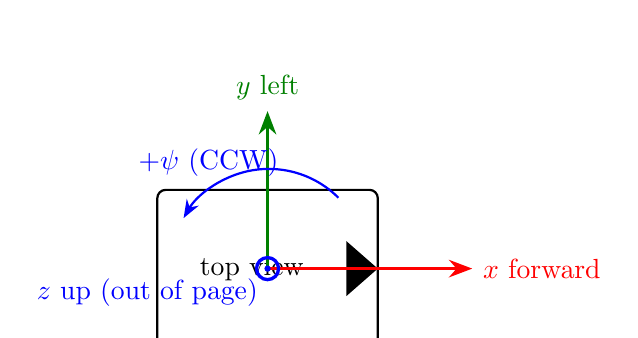
\begin{tikzpicture}[>=Stealth,scale=1.0]
  \draw[thick,rounded corners=3pt] (-1.4,-1.0) rectangle (1.4,1.0);
  \fill (1.4,0) -- (1.0,0.35) -- (1.0,-0.35) -- cycle;
  \node at (-0.2,0) {top view};
  \draw[->,very thick,red] (0,0) -- (2.6,0) node[right] {$x$ forward};
  \draw[->,very thick,green!50!black] (0,0) -- (0,2.0) node[above] {$y$ left};
  \draw[very thick,blue] (0,0) circle (0.14);
  \fill[blue] (0,0) circle (0.04);
  \node[blue,below left] at (0,0) {$z$ up (out of page)};
  \draw[->,thick,blue] (0.9,0.9) arc (45:150:1.25);
  \node[blue] at (-0.75,1.35) {$+\psi$ (CCW)};
\end{tikzpicture}
\caption{Body frame (FLU) seen from above. Rotation about $z$ is positive counter-clockwise.}\label{fig:frame}
\end{figure}

\begin{table}[H]
\centering
\caption{Expected signs. Right-hand rule about each axis: rotation about $+x$ lifts the left side, about $+y$ pitches the nose down, about $+z$ turns counter-clockwise.}\label{tab:signs}
\small
\begin{tabular}{@{}lccccc@{}}
\toprule
Motion & $a_x$ & $a_y$ & $a_z$ & Gyro axis & Gyro sign\\
\midrule
Nose up (front lifted) & $+$ & 0 & $\approx G\cos$ (slightly less) & $g_y$ & $-$\\
Left side up & 0 & $+$ & slightly less & $g_x$ & $+$\\
Turn counter-clockwise (flat) & 0 & 0 & $G$ & $g_z$ & $+$\\
Speeding up forwards (level) & $+$ & 0 & $G$ & -- & --\\
\bottomrule
\end{tabular}
\end{table}

For a robot at rest with roll $\phi$ and pitch $\theta$ (nose down positive), the specific force in the body frame is
\begin{equation}
  \begin{pmatrix}a_x\\a_y\\a_z\end{pmatrix}=G\begin{pmatrix}-\sin\theta\\ \cos\theta\sin\phi\\ \cos\theta\cos\phi\end{pmatrix}, \label{eq:gravity}
\end{equation}
so nose up (negative $\theta$) gives a positive $a_x$, and left side up gives a positive $a_y$, as in the table. Note that a stationary accelerometer reads $+G$ on the axis pointing up, not $-G$.

\section{Sensor configuration}
The driver writes only two registers; everything else keeps its power-on default. Table~\ref{tab:regs} lists the configuration that results.

\begin{table}[H]
\centering
\caption{MPU6050 configuration used by the driver. Values for the default registers and the filter bandwidths are from my recollection of the datasheet; please check them against it.}\label{tab:regs}
\small
\begin{tabular}{@{}llp{7.4cm}@{}}
\toprule
Register & Value & Effect\\
\midrule
\code{PWR\_MGMT\_1} (0x6B) & 0x00 & Wakes the chip, internal 8\,MHz oscillator as clock\\
\code{CONFIG} (0x1A) & 0x03 & Digital low-pass filter: about 44\,Hz accelerometer, 42\,Hz gyro, gyro output rate 1\,kHz\\
\code{GYRO\_CONFIG} (0x1B) & 0x00 (default) & $\pm250^\circ$/s, 131 LSB per $^\circ$/s\\
\code{ACCEL\_CONFIG} (0x1C) & 0x00 (default) & $\pm2\,g$, 16384 LSB per $g$\\
\code{SMPLRT\_DIV} (0x19) & not written & Internal sample rate not divided; the firmware simply reads the latest value\\
\bottomrule
\end{tabular}
\end{table}

One LSB of the gyro is $1/131=0.00763^\circ/\mathrm s=1.33\times10^{-4}$\,rad/s, and one LSB of the accelerometer is $6.0\times10^{-4}$\,m/s$^2$. Both are far below the noise, so quantisation of the raw data does not matter for heading.

\paragraph{Sampling and aliasing.} \code{main.cpp} reads the sensor every 50\,ms (20\,Hz) and the test firmware every 20\,ms (50\,Hz). Both rates have a Nyquist frequency (10\,Hz and 25\,Hz) below the 42\,Hz corner of the sensor's own filter, so vibration between those frequencies is aliased into the measured band instead of being removed. This adds noise but, being roughly zero-mean, no bias to the integral; Chapter~\ref{ch:limits} comes back to it.

\section{The driver \texttt{MPU6050\_Custom}}
Table~\ref{tab:driver} lists the driver's functions. The raw read is 14 bytes from register 0x3B in the order $a_x,a_y,a_z$, temperature, $g_x,g_y,g_z$, each a big-endian 16-bit integer; the driver stores them in \code{v[0..6]} so that the gyro is \code{v[4..6]} and \code{v[3]} (temperature) is read but never used.

\begin{table}[H]
\centering
\caption{Functions of \code{MPU6050\_Custom}.}\label{tab:driver}
\small
\begin{tabular}{@{}lp{10.4cm}@{}}
\toprule
Function & Behaviour\\
\midrule
\code{begin()} & Writes \code{PWR\_MGMT\_1}=0 and \code{CONFIG}=0x03; returns false only if the first write is not acknowledged\\
\code{readRaw(v)} & 14-byte burst read; false on any bus error\\
\code{calibrateGyro(400)} & Averages raw $g_z$ over 400 reads (3\,ms delay each) and stores it as \code{gyro\_bias\_z} in rad/s; only accepted if at least a quarter of the reads succeeded\\
\code{readData(\dots)} & Scales to SI units, subtracts the static offsets of Table~\ref{tab:offsets} and the runtime $g_z$ bias\\
\code{healthCheck()} & WHO\_AM\_I must be 0x68, 0x70, 0x71 or 0x72; the mean of 20 raw $|\mathbf a|$ readings must lie between 13100 and 19660 counts (0.8 to 1.2\,$g$); and $|\hat b_z|\le0.35$\,rad/s\\
\code{getGyroBiasZ()}, \code{updateGyroBiasZ()} & Access to the runtime $g_z$ bias, used by the ZUPT in \code{main.cpp}\\
\bottomrule
\end{tabular}
\end{table}

\subsection{Static offsets and scaling}
With $v_i$ the raw count, \code{readData} computes
\begin{align}
  a_x&=\tfrac{v_0}{16384}G-c_{ax}, & a_y&=\tfrac{v_1}{16384}G-c_{ay}, & a_z&=\tfrac{v_2}{16384}G-c_{az},\\
  g_x&=\tfrac{v_4}{131}\tfrac{\pi}{180}-c_{gx}, & g_y&=\tfrac{v_5}{131}\tfrac{\pi}{180}-c_{gy}, & g_z&=\tfrac{v_6}{131}\tfrac{\pi}{180}-\hat b_z, \label{eq:readdata}
\end{align}
with the constants of Table~\ref{tab:offsets}. These are the ``stage 1 resting offsets'' that the code comments refer to: values measured once, on one board, at one temperature, with the robot at rest. There is no scale correction for $g_z$ in the code, although a comment in \code{readData} still mentions a ``Stage 2 Z-axis scale factor (0.793)''; that comment is stale (Chapter~\ref{ch:limits}).

\begin{table}[H]
\centering
\caption{Static constants in \code{readData}. The measured value is the quantity subtracted, so for example $a_x$ gets $+0.377$\,m/s$^2$.}\label{tab:offsets}
\small
\begin{tabular}{@{}llll@{}}
\toprule
Channel & Constant & Value & Unit\\
\midrule
$a_x$ & $c_{ax}$ & $-0.377$ & m/s$^2$\\
$a_y$ & $c_{ay}$ & $0.211$ & m/s$^2$\\
$a_z$ & $c_{az}$ & $10.444-G=0.637$ & m/s$^2$\\
$g_x$ & $c_{gx}$ & $-0.04539$ (equal to $-2.60^\circ$/s) & rad/s\\
$g_y$ & $c_{gy}$ & $0.01483$ ($0.85^\circ$/s) & rad/s\\
$g_z$ & -- & measured at every boot by \code{calibrateGyro} & rad/s\\
\bottomrule
\end{tabular}
\end{table}

The $a_z$ constant tells us that this board's raw $z$ reading at rest is 10.444\,m/s$^2$, which is 6.5\,\% above $G$. The driver removes that excess as an offset, and \code{attitude.h} later removes any remaining gain error with a single factor (Chapter~\ref{ch:att}). One static pose cannot separate an offset from a gain error on $a_z$; Section~\ref{sec:accelcal} explains the consequence.

\section{Boot sequence}
\begin{figure}[H]
\centering
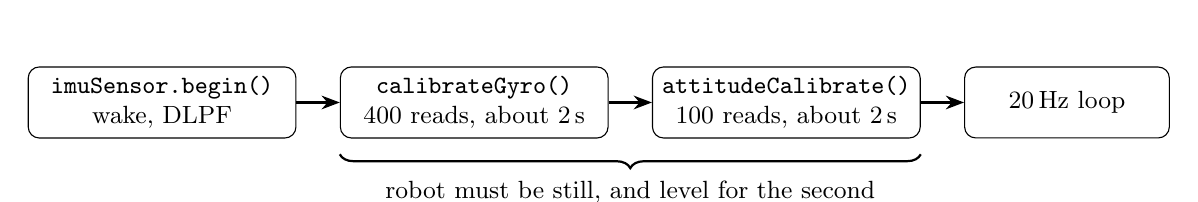
\begin{tikzpicture}[node distance=0.55cm,>=Stealth,
  b/.style={rectangle,draw,rounded corners,minimum width=3.4cm,minimum height=0.9cm,align=center,font=\small}]
  \node[b] (a) {\code{imuSensor.begin()}\\wake, DLPF};
  \node[b,right=of a] (c) {\code{calibrateGyro()}\\400 reads, about 2\,s};
  \node[b,right=of c] (d) {\code{attitudeCalibrate()}\\100 reads, about 2\,s};
  \node[b,right=of d,minimum width=2.6cm] (e) {20\,Hz loop};
  \draw[->,thick] (a) -- (c); \draw[->,thick] (c) -- (d); \draw[->,thick] (d) -- (e);
  \draw[decorate,decoration={brace,amplitude=5pt,mirror},thick] (c.south west)++(0,-0.2) -- ($(d.south east)+(0,-0.2)$) node[midway,below=6pt,font=\small] {robot must be still, and level for the second};
\end{tikzpicture}
\caption{Power-up sequence of the IMU in \code{setup()}. About four seconds of stillness are needed.}\label{fig:boot}
\end{figure}

The gyro calibration takes about 1.2\,s of delays plus the I$^2$C time of 400 reads, and the attitude calibration about 2\,s (100 reads with a 20\,ms delay). I estimate four seconds in total; I did not time it. If the robot is moved during either step, the bias or the zero attitude is wrong from then on (Section~\ref{sec:bootrisk}).

% ============================================================================
\chapter{Theory}
% ============================================================================

\section{Error model of a MEMS gyroscope}
A gyroscope channel measures
\begin{equation}
  \omega_{\mathrm{meas}}(t)=(1+s)\,\omega(t)+b(t)+n(t), \label{eq:gyromodel}
\end{equation}
where $s$ is the scale error, $b(t)$ a slowly varying bias and $n(t)$ white noise. Further terms exist (cross-axis misalignment, sensitivity to acceleration and vibration, temperature dependence of both $s$ and $b$), but for a robot that turns about a single axis on a flat floor the three terms above dominate. Integrating the corrected measurement over a time $T$ gives the heading error
\begin{equation}
  \hat\psi(T)-\psi(T)=s\,\psi(T)+\int_0^T\bigl(b-\hat b\bigr)\,dt+N_{\mathrm{ARW}}\,\sqrt T\,\xi,\qquad \xi\sim\mathcal N(0,1). \label{eq:yawerr}
\end{equation}
The first term grows with the angle turned, the second with time, and the third with the square root of time. Table~\ref{tab:gyroerr} gives the orders of magnitude for this robot.

\begin{table}[H]
\centering
\caption{Gyro error terms and their size for this robot. Datasheet figures are quoted as I remember them and must be checked; the measured values come from Chapter~\ref{ch:valid}.}\label{tab:gyroerr}
\small
\begin{tabular}{@{}p{3.2cm}p{4.6cm}p{6.2cm}@{}}
\toprule
Term & Datasheet (check) & This robot\\
\midrule
Scale error $s$ & about $\pm3\,\%$ tolerance & $+0.43\,\%$ measured, i.e.\ $1.5^\circ$ per turn\\
Zero-rate offset & about $\pm20^\circ$/s initially & removed at boot; the driver rejects $|b|>0.35$\,rad/s, which is $20^\circ$/s\\
Residual bias $b-\hat b$ & -- & $10^{-3}$\,rad/s gives $3.4^\circ$ per minute\\
Noise density & about $0.005^\circ/\mathrm s/\sqrt{\mathrm{Hz}}$ & $0.04^\circ$ after one minute: negligible\\
\bottomrule
\end{tabular}
\end{table}

\section{Bias estimation, ZUPT and dead-band}
\subsection{Boot-time estimate}
\code{calibrateGyro} averages $n=400$ raw readings of $g_z$. If the samples were independent with standard deviation $\sigma$, the error of the mean would be $\sigma/\sqrt{n}=\sigma/20$. The 42\,Hz hardware filter correlates neighbouring samples taken a few milliseconds apart, so the true error is somewhat larger. The estimate is only valid if the robot is still for those two seconds.

\subsection{Zero-velocity update}
In \code{main.cpp} the bias is refined while the robot is commanded to stand still. After one second of ``still'', and only while the corrected rate satisfies $|g_z|<0.05$\,rad/s, every 50\,ms sample updates
\begin{equation}
  \hat b_{k+1}=\hat b_k+\lambda\,g_{z,k},\qquad g_{z,k}=\text{raw}_k-\hat b_k,\quad\lambda=0.02, \label{eq:zupt}
\end{equation}
which is an exponential average of the raw readings with time constant $\Delta t/\lambda=2.5$\,s. For white noise of standard deviation $\sigma$ per sample, the estimate fluctuates around the truth with variance
\begin{equation}
  \operatorname{Var}(\hat b)=\frac{\lambda}{2-\lambda}\,\sigma^2\approx0.0101\,\sigma^2,\qquad \operatorname{std}(\hat b)\approx0.1\,\sigma. \label{eq:zuptvar}
\end{equation}
So the residual bias after a long stop is about a tenth of the per-sample noise. Stage~1 of the test prints that noise, which makes the figure checkable: with $\sigma=3\times10^{-3}$\,rad/s, $\operatorname{std}(\hat b)=3\times10^{-4}$\,rad/s and about 1$^\circ$ per minute of later motion.

Two properties of the gate matter. First, it is keyed on the \emph{commanded} state ($|v_{\mathrm{cmd}}|<0.003$\,m/s and $|\omega_{\mathrm{cmd}}|<0.01$\,rad/s), not on measured stillness, so a slow push below 0.05\,rad/s while the robot is commanded still is partly absorbed as bias. Second, the $|g_z|<0.05$\,rad/s condition means the loop can only \emph{refine} a boot calibration that is already within 0.05\,rad/s (2.9$^\circ$/s); if the boot estimate is worse than that, the update never runs (Section~\ref{sec:bootrisk}).

\subsection{Dead-band}
After the ZUPT, \code{main.cpp} sets $g_z=0$ whenever $|g_z|<0.005$\,rad/s ($0.29^\circ$/s). At rest this removes the integrated noise and the small residual bias, which is why the displayed yaw stays frozen. It has two costs: real rotation slower than $0.005$\,rad/s is lost (up to $17^\circ$ per minute), and, importantly for this report, the dead-band hides a residual bias only while the robot is still. During a turn $|g_z|$ is far above the threshold, so the bias is integrated in full. A yaw display that does not move at rest therefore does not prove that the bias is zero (Chapter~\ref{ch:valid}).

\section{Accelerometer tilt sensing}\label{sec:accelcal}
Inverting Equation~\eqref{eq:gravity} gives the tilt of a static robot:
\begin{equation}
  \phi_a=\operatorname{atan2}(a_y,\,a_z),\qquad \theta_a=\operatorname{atan2}\bigl(-a_x,\ \sqrt{a_y^2+a_z^2}\bigr), \label{eq:tiltacc}
\end{equation}
which are the expressions in \code{attitude.h}. The accuracy is limited by three things:
\begin{itemize}[noitemsep]
  \item \textbf{Offsets.} An offset $\delta$ on $a_x$ is a pitch error of $\delta/G$: $0.1$\,m/s$^2$ is $0.58^\circ$.
  \item \textbf{Linear acceleration.} Any acceleration along $x$ looks like pitch: $0.5$\,m/s$^2$ is $2.9^\circ$.
  \item \textbf{One-pose calibration.} The static offsets in Table~\ref{tab:offsets} come from a single resting pose. They absorb any tilt of the surface the robot stood on, and for $a_z$ they cannot separate offset from gain. A six-pose tumble would separate them; the single pose is adequate for a robot on mostly level floors.
\end{itemize}
An offset of 0.1\,m/s$^2$ also integrates to 0.1\,m/s of velocity error \emph{per second}, which is why the accelerometer is never integrated on its own here: the encoders correct the velocity and a ZUPT sets it to zero at rest (Chapter~\ref{ch:integration}).

\section{Euler-angle kinematics}
With body rates $p,q,r$ and ZYX Euler angles, the angle rates are
\begin{align}
  \dot\phi&=p+(q\sin\phi+r\cos\phi)\tan\theta,\\
  \dot\theta&=q\cos\phi-r\sin\phi,\\
  \dot\psi&=(q\sin\phi+r\cos\phi)/\cos\theta. \label{eq:euler}
\end{align}
\code{attitude.h} integrates the first two with a forward Euler step and leaves the third to the EKF. The term $\tan\theta$ is singular at $\theta=\pm90^\circ$, which a ground robot never approaches; at the 6$^\circ$ ramp threshold it is 0.105.

\section{The complementary filter}\label{sec:cf}
The gyro integral is accurate at short times and drifts at long times; the accelerometer angle is noisy and disturbed at short times and unbiased at long times. A first-order complementary filter weights them by frequency. With $\alpha=\tau/(\tau+\Delta t)$ one step is
\begin{equation}
  \hat x_{k+1}=\alpha\,\bigl(\hat x_k+\omega_k\,\Delta t\bigr)+(1-\alpha)\,x_{a,k}. \label{eq:cf}
\end{equation}
In continuous time this is a low-pass filter $1/(\tau s+1)$ on the accelerometer angle plus a high-pass filter $\tau s/(\tau s+1)$ on the integrated gyro, which add to one. The crossover is at
\begin{equation}
  f_c=\frac{1}{2\pi\tau}=0.159\ \mathrm{Hz}\quad(\tau=1\ \mathrm s),\qquad \alpha=0.952\ \ (\Delta t=0.05\ \mathrm s). \label{eq:fc}
\end{equation}

\begin{figure}[H]
\centering
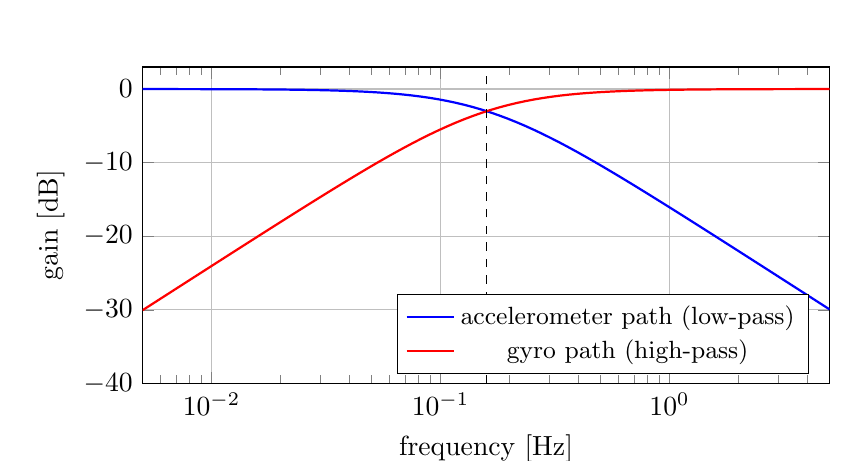
\begin{tikzpicture}
\begin{axis}[width=0.85\textwidth,height=5.6cm,xmode=log,xlabel={frequency [Hz]},ylabel={gain [dB]},grid=major,xmin=0.005,xmax=5,ymin=-40,ymax=3,legend pos=south east,legend style={font=\small},samples=80,domain=0.005:5]
\addplot[thick,blue] {-10*ln(1+(2*pi*x*1.0)^2)/ln(10)};
\addplot[thick,red] {10*ln((2*pi*x*1.0)^2/(1+(2*pi*x*1.0)^2))/ln(10)};
\draw[dashed] (axis cs:0.159,-40) -- (axis cs:0.159,3);
\legend{accelerometer path (low-pass),gyro path (high-pass)}
\end{axis}
\end{tikzpicture}
\caption{Magnitude of the two paths of the complementary filter for $\tau=1$\,s. They cross at 0.159\,Hz (dashed), where each contributes $-3$\,dB.}\label{fig:cfbode}
\end{figure}

\subsection{Effect of a gyro bias}
With a constant residual rate bias $b$ on the gyro and a true angle of zero, Equation~\eqref{eq:cf} settles at
\begin{equation}
  \hat x_\infty=\frac{\alpha\,b\,\Delta t}{1-\alpha}=\tau\,b, \label{eq:cfbias}
\end{equation}
exactly, for any $\Delta t$. A bias of $0.01$\,rad/s therefore costs $0.57^\circ$ of roll or pitch. The Python replica of \code{attitude.h} (Chapter~\ref{ch:valid}) reproduces this to six digits. \code{attitude.h} subtracts a boot-time mean for $g_x$ and $g_y$ and never updates it afterwards, so a drift of those two biases with temperature enters roll and pitch as $\tau\,\Delta b$.

\subsection{Accelerometer gating}
When the measured magnitude differs from $G$ by more than 15\,\%, i.e.\ $|\lVert\mathbf a\rVert-G|\ge0.147\,G=1.47$\,m/s$^2$, the filter sets $\alpha=1$ and runs on the gyro alone. That catches bumps and impacts. It does not catch the accelerations this robot produces: at its top speed of 0.48\,m/s the accelerations are a few tenths of m/s$^2$, well inside the gate. Those leak into the pitch estimate, as the next section shows.

\section{Gravity compensation and its side effect}\label{sec:leak}
The forward acceleration used by the EKF is the measured $a_x$ with the gravity component of Equation~\eqref{eq:gravity} removed:
\begin{equation}
  a_{\mathrm{fwd}}=a_x+G\sin\hat\theta. \label{eq:afwd}
\end{equation}
This is correct if $\hat\theta$ is the true pitch. But $\hat\theta$ is itself corrected by the accelerometer angle $\theta_a=\operatorname{atan2}(-a_x,\dots)$, which includes the robot's own acceleration. Under a sustained forward acceleration $a$ on a level floor the filter output tends to $\hat\theta\to-(a/G)\,(1-e^{-t/\tau})$, and then
\begin{equation}
  a_{\mathrm{fwd}}\approx a\,e^{-t/\tau}. \label{eq:leak}
\end{equation}
The compensated acceleration is the true one passed through a high-pass filter with time constant $\tau=1$\,s. Integrated, it can deliver at most $a\tau$ of velocity, however long the acceleration lasts; and when the acceleration ends, the pitch estimate still holds the leaked angle, so $a_{\mathrm{fwd}}$ goes negative and cancels most of what was gained. Figure~\ref{fig:leak} shows the result for $a=0.3$\,m/s$^2$ applied for four seconds.

\begin{figure}[H]\centering
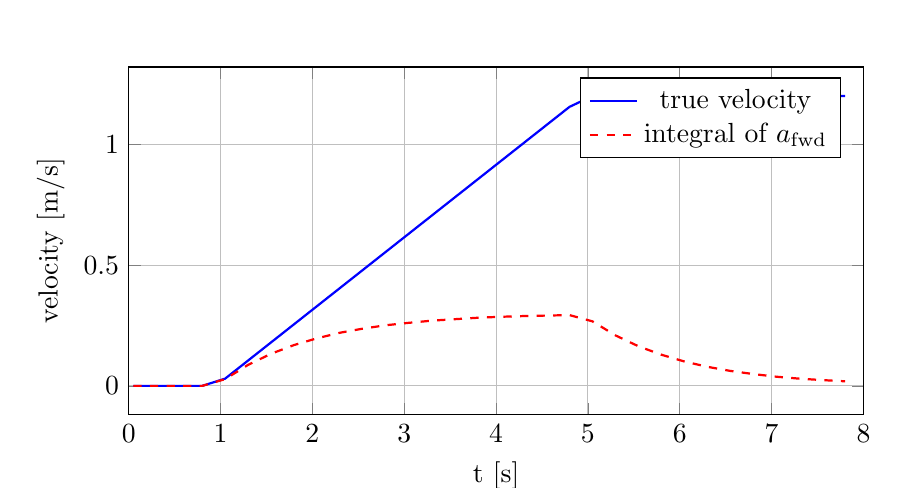
\begin{tikzpicture}
\begin{axis}[width=0.9\textwidth,height=6cm,xlabel={t [s]},ylabel={velocity [m/s]},legend pos=north east,grid=major,xmin=0,xmax=8]
\addplot[thick,blue] coordinates {(0.05,0.0) (0.3,0.0) (0.55,0.0) (0.8,0.0) (1.05,0.03) (1.3,0.105) (1.55,0.18) (1.8,0.255) (2.05,0.33) (2.3,0.405) (2.55,0.48) (2.8,0.555) (3.05,0.63) (3.3,0.705) (3.55,0.78) (3.8,0.855) (4.05,0.93) (4.3,1.005) (4.55,1.08) (4.8,1.155) (5.05,1.2) (5.3,1.2) (5.55,1.2) (5.8,1.2) (6.05,1.2) (6.3,1.2) (6.55,1.2) (6.8,1.2) (7.05,1.2) (7.3,1.2) (7.55,1.2) (7.8,1.2)};\addlegendentry{true velocity}
\addplot[thick,red,dashed] coordinates {(0.05,0.0) (0.3,0.0) (0.55,0.0) (0.8,0.0) (1.05,0.028) (1.3,0.087) (1.55,0.133) (1.8,0.169) (2.05,0.197) (2.3,0.22) (2.55,0.237) (2.8,0.251) (3.05,0.261) (3.3,0.27) (3.55,0.276) (3.8,0.282) (4.05,0.286) (4.3,0.289) (4.55,0.291) (4.8,0.293) (5.05,0.267) (5.3,0.209) (5.55,0.164) (5.8,0.129) (6.05,0.101) (6.3,0.079) (6.55,0.062) (6.8,0.049) (7.05,0.038) (7.3,0.03) (7.55,0.024) (7.8,0.019)};\addlegendentry{integral of $a_{\mathrm{fwd}}$}
\end{axis}\end{tikzpicture}
\caption{Simulation: velocity from integrating the compensated forward acceleration (dashed) against the true velocity, for 0.3\,m/s$^2$ applied between 1 and 5\,s.}\label{fig:leak}
\end{figure}

The consequence is limited by design: the EKF takes velocity mostly from the encoders (measurement noise 0.02 against process noise 0.05 for the velocity state), so the accelerometer acts only as a short-term predictor. But the accelerometer should not be relied on to supply speed during sustained acceleration, and its published \code{linear\_acceleration} is the raw measurement scaled by $k$, not this compensated value.

\section{Heading integration and the EKF}
The EKF state is $[x,\,y,\,\psi,\,v]$. The prediction step advances the heading with $\psi\leftarrow\psi+g_z\,\Delta t$ and the measurement step compares predicted position, heading and velocity with encoder-derived values. For heading, \code{main.cpp} forces the innovation to zero (\code{Y(2) = 0}), with the comment that skid-steer encoders under-read turns. One could still ask whether the encoders can influence heading indirectly, through cross-covariances in $P$ and the velocity innovation. The Python replica of the EKF block (Chapter~\ref{ch:valid}) says they do not in any measurable way: over 60\,s of driving at 0.2\,m/s, with a noisy encoder and with turn rates of 0, 0.3 and $-1.0$\,rad/s, the EKF heading never differed from the pure integral of $g_z$ by more than $1.2\times10^{-6}$\,rad. So Equation~\eqref{eq:yawerr} is the complete heading error budget.

\section{Error budget}
Table~\ref{tab:budget} turns the models above into numbers for a single turn and for a minute of driving. The right-hand column uses the values measured in Chapter~\ref{ch:valid}.

\begin{table}[H]
\centering
\caption{Heading error budget. $\psi$ is the angle turned and $T$ the elapsed time.}\label{tab:budget}
\small
\begin{tabular}{@{}p{3.6cm}p{4.2cm}p{6.2cm}@{}}
\toprule
Source & Formula & Example\\
\midrule
Scale error & $s\,\psi$ & $0.43\,\%$: $1.5^\circ$ per $360^\circ$\\
Residual bias & $(b-\hat b)\,T$ & $1.1\times10^{-3}$\,rad/s: $3.9^\circ$ in 60\,s\\
Noise (ARW) & $N_{\mathrm{ARW}}\sqrt T$ & $0.04^\circ$ in 60\,s\\
ZUPT jitter & $0.1\,\sigma\,T$ & $\sigma=3\times10^{-3}$\,rad/s: $1^\circ$ per minute of motion\\
Dead-band loss & up to $0.005\,T$ & only for rotation slower than $0.29^\circ$/s\\
\bottomrule
\end{tabular}
\end{table}

Scan matching in the SLAM stack absorbs errors of this size as long as the scene has structure to match, so none of these terms needs to be eliminated, but the scale and bias terms are the ones worth measuring because they are systematic.

% ============================================================================
\chapter[Test Firmware]{Test Firmware: \texttt{IMU\_CALIBRATE.cpp}}\label{ch:test}
% ============================================================================

\section{Purpose and design}
\code{IMU\_CALIBRATE.cpp} is a guided test. The terminal tells the operator what to do and when, the firmware measures, and it prints a set of lines that all begin with \code{RESULT}. The operator copies those lines and nothing else needs to be recorded. It is flashed \emph{instead of} \code{main.cpp}, contains no motor or ROS code, and uses the same \code{MPU6050\_Custom} driver as the robot.

That last point shapes what the test measures. Because it calls \code{readData}, every value it prints is \emph{after} the driver's static offsets of Table~\ref{tab:offsets}. It therefore measures the \emph{residual} with respect to the stored constants, not the raw sensor output, and it does not call \code{calibrateGyro}, so its $g_z$ is the raw reading with the runtime bias at its initial value of zero. Section~\ref{sec:updateconst} turns these residuals into new constants.

The test has four stages and takes about two minutes:
\begin{enumerate}[noitemsep]
  \item \textbf{Still} (8\,s): offsets, noise, gyro bias, apparent mounting tilt.
  \item \textbf{Spin} (30\,s window): one full counter-clockwise turn by hand; gyro sign and scale.
  \item \textbf{Nose up}: accelerometer against gyro on the pitch axis.
  \item \textbf{Left side up}: accelerometer against gyro on the roll axis.
\end{enumerate}

\section{Building and flashing}
The header comment of the file gives the PlatformIO environment. With the file's actual name it reads:
\begin{lstlisting}[language=bash]
[env:imu_test]
extends = env:<your existing env>
build_src_filter = -<*> +<IMU_CALIBRATE.cpp> +<MPU6050_Custom.cpp>
\end{lstlisting}
The header comment still says \code{imu\_guided\_test.cpp}; if you copy the filter from there, the build finds no source file. The program needs \code{pins.h} and the driver from the project, and the serial monitor must be at 115200\,baud. The prompt ``press ENTER when ready'' is satisfied by \emph{any} received byte, so the monitor must be set to send a line ending (or any key) when you press Enter.

\section{Constants and data structures}
\begin{table}[H]
\centering
\caption{Constants and state in \code{IMU\_CALIBRATE.cpp}.}\label{tab:testconst}
\small
\begin{tabular}{@{}lp{10cm}@{}}
\toprule
Name & Meaning\\
\midrule
\code{SAMPLE\_US} = 20000 & Sample period, 20\,ms (50\,Hz)\\
\code{DUMP\_RAW} = 0 & If 1, every sample is also streamed as \code{RAW,stage,millis,ax,ay,az,gx,gy,gz}; produces long output\\
\code{struct Win} & One recording window: count $n$, sums and sums of squares of the six channels, and the integral of (gyro $-$ bias) about each axis\\
\code{bias[3]} & Gyro means from Stage~1 (rad/s); subtracted in the gyro integrals of the later stages\\
\code{stageNo} & Stage number, used only for the raw dump\\
\bottomrule
\end{tabular}
\end{table}

\section{Sampling and statistics}
\code{collect(ms, w)} polls in a loop with a 1\,ms delay and takes a sample as soon as 20\,ms have passed since the previous one, so the actual period is 20 to 21\,ms. If a read fails it waits 1\,ms and tries again; the interval used for integration is always the \emph{measured} one, taken from \code{micros()}, so a failed read lengthens one step but does not bias the integral. For each accepted sample $i$ with measured interval $\Delta t_i$:
\begin{align}
  \bar x_c&=\frac1n\sum_i x_{c,i}, & \sigma_c&=\sqrt{\frac1n\sum_i x_{c,i}^2-\bar x_c^{\,2}}, & \Theta_k&=\sum_i\bigl(g_{k,i}-\beta_k\bigr)\Delta t_i, \label{eq:stats}
\end{align}
where $c$ runs over the six channels, $\beta_k$ is the Stage-1 bias of gyro axis $k$ and $\Theta_k$ the integrated angle. The standard deviation is the population form and is computed in double precision from float inputs, which is adequate for these magnitudes. The integral is a rectangular sum with each sample weighted by the interval that ends at it.

\section{Start-up probes}
Before the stages, \code{setup()} identifies the chip and probes its registers. These lines are the quickest way to find out whether a board sold as an MPU6050 is one.

\begin{table}[H]
\centering
\caption{Start-up probe lines and their interpretation. Register behaviour is from my recollection of the datasheets and register maps; check them.}\label{tab:probes}
\small
\begin{tabular}{@{}p{4.2cm}p{9.6cm}@{}}
\toprule
Line & Meaning\\
\midrule
\code{WHO\_AM\_I=0x68} & A genuine MPU6050. 0x70 and 0x71 are the MPU-6500 and MPU-9250 families, and 0x72 appears on some clones. \code{healthCheck} accepts all four, so it does not distinguish them\\
\code{WHO\_AM\_I read FAILED} & No acknowledge at 0x68: wiring, power, or the address pin is high (address 0x69)\\
\code{GYRO\_CONFIG}, \code{ACCEL\_CONFIG} & Should both be 0x00 (full scale $\pm250^\circ$/s and $\pm2\,g$, matching the 131 and 16384 divisors in the driver)\\
\code{ACCEL\_CONFIG2 (1D)} readback after writing 0x03 & \code{0x00} suggests no such register, as on a real MPU6050; \code{0x03} means the chip implements \code{ACCEL\_CONFIG2}, i.e.\ it is in the MPU-6500 family. In that case the accelerometer filter is set by register 0x1D, which \code{begin()} never writes\\
\code{imu.begin() FAILED} & The wake-up write was not acknowledged; the test stops\\
\bottomrule
\end{tabular}
\end{table}
The probe writes \code{PWR\_MGMT\_1}=0x01 before reading, then restores 0x1D to 0x00; afterwards \code{imu.begin()} writes \code{PWR\_MGMT\_1}=0 again, so the sensor is left in the driver's normal configuration for the stages.

\section{Stage 1: still}\label{sec:s1}
\paragraph{Procedure.} The robot rests flat on a level surface, wheels down; after a three-second countdown the firmware records for 8\,s while the operator does not touch the robot or the table.

\paragraph{Computation.} The window means of the gyro channels become the bias used by every later stage. The program prints the sample count (about 390 to 400), the mean accelerometer vector and its magnitude, the accelerometer standard deviations, the gyro means and standard deviations, and two mounting angles computed from the mean accelerometer vector:
\begin{equation}
  \text{climb}=\operatorname{atan2}\bigl(\bar a_x,\sqrt{\bar a_y^2+\bar a_z^2}\bigr),\qquad
  \text{leftUp}=\operatorname{atan2}(\bar a_y,\,\bar a_z). \label{eq:climb}
\end{equation}
They are positive for nose up and left side up respectively, i.e.\ the opposite sign to the pitch of Equation~\eqref{eq:tiltacc} (climb equals $-\theta_a$). On a level surface both should be near zero; a nonzero value is a mount tilt, a tilted table, or an accelerometer offset, and the test cannot tell which.

\paragraph{What the numbers mean.} With the static offsets applied, $\bar a_x\approx\bar a_y\approx0$ and $\bar a_z\approx G$, and $\lVert\bar{\mathbf a}\rVert\approx G$; deviations are residual offsets, or a gain error if the magnitude is wrong. The gyro means for $x$ and $y$ are the residuals relative to $c_{gx},c_{gy}$ and should be small. The $z$ mean is the board's actual zero-rate output, which \code{calibrateGyro} re-measures at each boot. The three gyro standard deviations are the noise figure used in Equation~\eqref{eq:zuptvar}. If any exceeds 0.01\,rad/s the firmware prints a warning that the robot was moving or vibrating and the stage must be repeated.

\section{Stage 2: spin}\label{sec:s2}
\paragraph{Procedure.} The operator marks the robot's nose on the surface, then, after the countdown, turns the robot \emph{one full turn counter-clockwise} seen from above, flat and smoothly, in about 6 to 10\,s, ends exactly on the mark and holds still until ``STOP''. The recording window is 30\,s regardless.

\paragraph{Computation.} The $z$ integral of Equation~\eqref{eq:stats} is the angle $\Theta_z$ the gyro reports for what should be $+360^\circ$:
\begin{equation}
  \Theta_z=\sum_i\bigl(g_{z,i}-\beta_z\bigr)\Delta t_i,\qquad S_{\mathrm{rep}}=\frac{|\Theta_z|}{360^\circ}. \label{eq:s2scale}
\end{equation}
The printed ``gyro scale factor'' is $S_{\mathrm{rep}}$, the ratio of \emph{reported to true} rotation. A value above 1 means the gyro over-reads, and the correction to apply is its reciprocal. The sign line says that $\Theta_z>0$ for a counter-clockwise turn means the frame is standard (FLU), and a negative value means the axis is inverted. The program also prints the $x$ and $y$ integrals, which should be near zero for a flat turn, and warns if $|\Theta_z|$ is outside 270 to 450$^\circ$.

\paragraph{Resolution.} One turn cannot resolve a scale error as small as the one measured on this robot. Three effects each contribute: the operator's alignment on the mark ($\pm1$ to $2^\circ$, i.e.\ $\pm0.3$ to $0.5\,\%$ of 360$^\circ$); the residual bias integrated over the 30\,s window ($10^{-3}$\,rad/s gives $1.7^\circ$, or $0.5\,\%$); and the extra rotation or lag at the start and end. Together they are of the order of $\pm0.7\,\%$. The stage is excellent for the \emph{sign} and for catching a gross scale error, but to measure the scale to a few tenths of a percent use the multi-turn protocol of Section~\ref{sec:multiturn}.

\section{Stages 3 and 4: tilt}
\paragraph{Procedure.} The robot lies flat; after the countdown the operator holds it flat for 3\,s, lifts the front (stage 3) or the left side (stage 4) by about 15 to 20$^\circ$ over 4\,s, and holds the raised angle for 3\,s. A book under the front or the left wheels is convenient.

\paragraph{Computation.} With the accelerometer angle $A$ taken from Equation~\eqref{eq:climb} (climb for stage 3, leftUp for stage 4), the program computes the change between the flat and the held windows, $\Delta A=A_{\mathrm{hold}}-A_{\mathrm{flat}}$, and compares it with the gyro integral over the lift and the hold windows, in the same sign convention:
\begin{align}
  \text{stage 3: } G_\theta&=-\frac{180^\circ}{\pi}\bigl(\Theta_y^{\mathrm{lift}}+\Theta_y^{\mathrm{hold}}\bigr), &
  \text{stage 4: } G_\phi&=+\frac{180^\circ}{\pi}\bigl(\Theta_x^{\mathrm{lift}}+\Theta_x^{\mathrm{hold}}\bigr),
\end{align}
and prints the ratio $G/\Delta A$ if $|\Delta A|>1^\circ$. The minus sign in stage 3 is there because nose up is a negative rotation about $+y$. It also prints the changes of the three accelerometer means, the gyro standard deviations while holding, and two warnings: ``tilt under 8$^\circ$'' and ``SIGN MISMATCH between accel and gyro''.

\paragraph{Expected values.} For a lift angle $\beta$ the accelerometer changes by
\begin{equation}
  \Delta a_{\mathrm{lift}}\approx G\sin\beta,\qquad \Delta a_z\approx G(\cos\beta-1), \label{eq:tiltexp}
\end{equation}
with $\Delta a_{\mathrm{lift}}=\Delta a_x$ in stage 3 and $\Delta a_y$ in stage 4. For $\beta=15^\circ$ these are $+2.54$ and $-0.33$\,m/s$^2$; for $20^\circ$, $+3.35$ and $-0.59$\,m/s$^2$. The gyro/accelerometer ratio should be close to 1. This stage exists to prove that the gyro and accelerometer agree in \emph{sign and gain}, which the complementary filter of Chapter~\ref{ch:att} depends on: a sign error in either would make the filter pull the estimate away from the truth instead of toward it.

\section{Output reference}
\begin{table}[H]
\centering
\caption{The \code{RESULT} lines, in the order they appear.}\label{tab:resultlines}
\small
\begin{tabular}{@{}p{3.4cm}p{6.2cm}p{4.2cm}@{}}
\toprule
Line & Content & Use\\
\midrule
\code{WHO\_AM\_I}, \code{REG} & Chip identity and register values (Table~\ref{tab:probes}) & Genuine-part check\\
\code{S1 samples} & Sample count in 8\,s & Check about 390--400\\
\code{S1 accel mean} & $\bar a_x,\bar a_y,\bar a_z$ and $\lVert\bar{\mathbf a}\rVert$ & Offset constants, gain check\\
\code{S1 accel std} & $\sigma$ per accelerometer axis & Noise\\
\code{S1 gyro bias} & $\beta_x,\beta_y,\beta_z$ & Gyro offset constants\\
\code{S1 gyro std} & $\sigma$ per gyro axis & Input to Equation~\eqref{eq:zuptvar}\\
\code{S1 apparent climb} & Mount tilt (climb, leftUp) & Level check\\
\code{S2 gz integral} & $\Theta_z$ for one CCW turn & Scale\\
\code{S2 gyro scale factor} & $S_{\mathrm{rep}}$, reported over true & Scale (take reciprocal to correct)\\
\code{S2 gx,gy integrals} & Cross-axis leakage & Mounting\\
\code{S2 verdict} & Sign of $g_z$ for CCW & Frame check\\
\code{S3/S4 accel angle} & Flat and raised angle, change & Tilt actually applied\\
\code{S3/S4 gyro integral} & $G_\theta$ or $G_\phi$ & Agreement with accelerometer\\
\code{S3/S4 ratio} & $G/\Delta A$ & Should be near 1\\
\code{S3/S4 raised-minus-flat} & $\Delta a_x,\Delta a_y,\Delta a_z$ & Compare with Eq.~\eqref{eq:tiltexp}\\
\code{S3/S4 gyro std} & Noise while holding & Hand steadiness\\
\bottomrule
\end{tabular}
\end{table}

After the last stage the program prints ``ALL DONE''; pressing any key restarts the board for another run (\code{loop()} calls \code{ESP.restart()} on the first received byte).

% ============================================================================
\chapter[Attitude Filter]{The Attitude Filter: \texttt{attitude.h}}\label{ch:att}
% ============================================================================

\section{Interface}
\code{attitude.h} is a small header-only class that estimates roll and pitch, provides gravity-compensated forward acceleration and flags a ramp. Table~\ref{tab:attif} lists its members.

\begin{table}[H]
\centering
\caption{Public interface of the \code{Attitude} class.}\label{tab:attif}
\small
\begin{tabular}{@{}lp{9.8cm}@{}}
\toprule
Member & Description\\
\midrule
\code{roll}, \code{pitch} & Estimates in radians; pitch positive nose down, roll positive left side up\\
\code{ramp} & True while the robot is judged to be on a ramp\\
\code{calibrate(a[3], g[3])} & Sets the accelerometer gain, the gyro $x,y$ bias and the zero attitude from still averages\\
\code{update(ax,ay,az,gx,gy,gz,dt)} & One filter step (Section~\ref{sec:attupdate})\\
\code{forwardAccel()} & $a_x+G\sin\theta$, the gravity-compensated forward acceleration\\
\code{gainK()} & The accelerometer gain correction $k$\\
\code{gyroBias(i)} & The stored bias of gyro axis $i$ (the $z$ entry is always 0)\\
\bottomrule
\end{tabular}
\end{table}

\section{Calibration}
\code{calibrate} receives the mean accelerometer vector $\mathbf a$ and mean gyro vector $\mathbf g$ over a still period (100 samples in \code{attitudeCalibrate}, taken from \code{readData} so the static offsets are already applied).
\begin{align}
  k&=\frac{G}{\lVert\mathbf a\rVert}, & \hat b_x&=\bar g_x, & \hat b_y&=\bar g_y, & \hat b_z&=0, \label{eq:attcal}\\
  \theta_0&=\operatorname{atan2}\bigl(-ka_x,\sqrt{(ka_y)^2+(ka_z)^2}\bigr), & \phi_0&=\operatorname{atan2}(ka_y,\,ka_z), & \phi&=\theta=0.
\end{align}
The factor $k$ is a single-point correction of the accelerometer gain, applied to all three axes at every update and also to the published \code{linear\_acceleration}. The offsets $\theta_0,\phi_0$ define the robot's pose at boot as zero roll and zero pitch, so a robot that boots on a slope reports zero tilt there and its pitch is relative to that slope. The $z$ bias is left to the driver and the ZUPT.

\section{The update step}\label{sec:attupdate}
Each call performs the following, with $p=g_x-\hat b_x$, $q=g_y-\hat b_y$, $r=g_z$ (already corrected by the driver):
\begin{enumerate}[noitemsep]
  \item Scale the accelerometer by $k$ and store the scaled $a_x$ for \code{forwardAccel}.
  \item Integrate the Euler rates of Equation~\eqref{eq:euler}: $\phi_G=\phi+(p+(q\sin\phi+r\cos\phi)\tan\theta)\Delta t$ and $\theta_G=\theta+(q\cos\phi-r\sin\phi)\Delta t$.
  \item Compute the accelerometer angles, $\phi_A=\operatorname{atan2}(a_y,a_z)-\phi_0$ and $\theta_A=\operatorname{atan2}(-a_x,\sqrt{a_y^2+a_z^2})-\theta_0$.
  \item Choose the weight: $\alpha=\tau/(\tau+\Delta t)$ if $|\lVert\mathbf a\rVert-G|<0.15\,G$, otherwise $\alpha=1$.
  \item Blend: $\phi\leftarrow\alpha\phi_G+(1-\alpha)\phi_A$, and the same for $\theta$.
  \item Update the ramp flag (next section).
\end{enumerate}
Listing~\ref{lst:attupdate} shows the corresponding code.

\begin{lstlisting}[language=C++,caption={Core of \texttt{Attitude::update()}.},label={lst:attupdate}]
float p = gx - gb_[0], q = gy - gb_[1], r = gz;
float sr = sinf(roll), cr = cosf(roll), tp = tanf(pitch);
float rollG  = roll  + (p + (q*sr + r*cr)*tp) * dt;
float pitchG = pitch + (q*cr - r*sr) * dt;

float n = sqrtf(ax*ax + ay*ay + az*az);
float alpha = (fabsf(n - G) < 0.15f*G) ? TAU/(TAU + dt) : 1.0f;
float rollA  = atan2f(ay, az) - roll0_;
float pitchA = atan2f(-ax, hypotf(ay, az)) - pitch0_;
roll  = alpha*rollG  + (1.0f - alpha)*rollA;
pitch = alpha*pitchG + (1.0f - alpha)*pitchA;
\end{lstlisting}

\begin{table}[H]
\centering
\caption{Constants in \code{attitude.h}.}\label{tab:attconst}
\small
\begin{tabular}{@{}llp{7cm}@{}}
\toprule
Name & Value & Role\\
\midrule
\code{G} & 9.80665\,m/s$^2$ & Gravity\\
\code{TAU} & 1.0\,s & Complementary-filter time constant; $f_c=0.159$\,Hz\\
gate & $0.15\,G$ & Accelerometer magnitude window for blending\\
\code{RAMP\_ON} & 0.1047\,rad ($6.0^\circ$) & $|\theta|$ above this starts the ramp timer\\
\code{RAMP\_OFF} & 0.0698\,rad ($4.0^\circ$) & $|\theta|$ below this starts the release timer\\
debounce & 0.3\,s & Time a condition must hold before the flag changes\\
\bottomrule
\end{tabular}
\end{table}

\section{Ramp detection}
The ramp flag is a hysteresis comparator on $|\theta|$ with a debounce timer. While the flag is false, a timer accumulates $\Delta t$ for as long as $|\theta|>6^\circ$ and is reset to zero otherwise; after 0.3\,s the flag becomes true. While it is true, the timer accumulates for as long as $|\theta|<4^\circ$, and the flag clears after 0.3\,s. The 2$^\circ$ hysteresis and the 0.3\,s debounce keep the flag from chattering when the pitch estimate hovers near a threshold. In the supplied \code{main.cpp} the flag is computed but not read anywhere, so it currently has no effect on behaviour.

\section{Behaviour checked by simulation}
A Python replica of the class, written line by line from the header, was used to test three properties. They are simulations of the filter with ideal sensors, not measurements.
\begin{itemize}[noitemsep]
  \item \textbf{Tracking.} With a gyro and accelerometer consistent with a 10$^\circ$ nose-up ramp over one second, the pitch estimate follows the truth with no error beyond numerical precision, as expected when sensors agree.
  \item \textbf{Bias.} A residual rate bias $b$ on $g_y$ with a still, level robot settles at the pitch error $\tau b$ predicted by Equation~\eqref{eq:cfbias} (Table~\ref{tab:attbias}).
  \item \textbf{Acceleration leakage.} Equation~\eqref{eq:leak}, shown in Figure~\ref{fig:leak}.
\end{itemize}
The weight $\alpha$ also depends on the sample period: 0.980 at the test firmware's 20\,ms, 0.952 at the robot's 50\,ms, and 0.909 if a step were stretched to 100\,ms. The filter is not sensitive to this.

\begin{table}[H]
\centering
\caption{Steady-state pitch error caused by a residual gyro bias (level, still robot, $\tau=1$\,s). The simulated value equals the prediction $\tau b$.}\label{tab:attbias}
\small
\begin{tabular}{@{}ccc@{}}
\toprule
Residual bias $b$ [rad/s] & Predicted $\tau b$ [deg] & Simulated [deg]\\
\midrule
0.001 & 0.057 & 0.057 \\
0.002 & 0.115 & 0.115 \\
0.005 & 0.286 & 0.286 \\
0.010 & 0.573 & 0.573 \\
\bottomrule
\end{tabular}
\end{table}

\section{Limitations}
\begin{itemize}[noitemsep]
  \item Forward-Euler integration of the angles is adequate at 20\,Hz for the small angles of a ground robot but would not be for fast, large rotations.
  \item $\tan\theta$ is singular at $\pm90^\circ$; harmless here.
  \item The $x$ and $y$ gyro biases are measured once at boot and never updated.
  \item The accelerometer is calibrated at one pose: gain and offset on each axis cannot be separated.
  \item The gate of 15\,\% of $G$ does not exclude the robot's own accelerations (Section~\ref{sec:leak}).
  \item The estimate has no yaw; the heading comes from the EKF.
\end{itemize}

% ============================================================================
\chapter[Integration in main.cpp]{Integration in \texttt{main.cpp}}\label{ch:integration}
% ============================================================================

\section{Boot}
The relevant part of \code{setup()} is
\begin{lstlisting}[language=C++,caption={IMU start-up in \texttt{setup()}.},label={lst:boot}]
if (imuSensor.begin()) {
  imu_active = true;
  imuSensor.calibrateGyro();   // robot must be still (~1.2 s)
  attitudeCalibrate();         // robot must be still and level (~2 s)
  last_filter_us = micros();
}
\end{lstlisting}
\code{attitudeCalibrate} reads 100 samples 20\,ms apart through \code{readData}, averages them, and hands the means to \code{att.calibrate}. It returns without calibrating if fewer than 50 reads succeeded, in which case \code{k\_} stays at 1 and the zero offsets at 0.

\section{Processing order in the 20\,Hz loop}
Every 50\,ms \code{loop()} runs the block of Table~\ref{tab:order} when a sample is available and the interval is between 0 and 0.5\,s.

\begin{table}[H]
\centering
\caption{Order of operations on each IMU sample in \code{main.cpp}.}\label{tab:order}
\small
\begin{tabular}{@{}cp{5.2cm}p{7.2cm}@{}}
\toprule
\# & Step & Detail\\
\midrule
1 & \code{readData} & Driver-corrected $a$ and $g$; $g_z$ has the runtime bias removed\\
2 & $\Delta t$ from \code{micros()} & Used by every later step\\
3 & \code{att.update(\dots)} & Receives $g_z$ \emph{before} the ZUPT and dead-band, so roll and pitch are unaffected by them\\
4 & Still detection & Commanded velocity below 0.003\,m/s and commanded turn rate below 0.01\,rad/s\\
5 & ZUPT & After 1\,s of ``still'' and with $|g_z|<0.05$\,rad/s: update the bias by $0.02\,g_z$ and remove the same amount from this sample\\
6 & Dead-band & $|g_z|<0.005$\,rad/s becomes 0\\
7 & Encoder deltas & Wheel distances; used for the velocity measurement\\
8 & EKF prediction & $\psi\leftarrow\psi+g_z\Delta t$; $v\leftarrow v+a_{\mathrm{fwd}}\Delta t$ (forced to 0 when ``still'')\\
9 & EKF update & Heading innovation forced to zero; velocity corrected by the encoders\\
10 & Heading hold & Uses $\psi$ and $g_z$ when active\\
11 & Publish & \code{/imu\_data} and \code{/odometry/filtered}\\
\bottomrule
\end{tabular}
\end{table}

\section{ZUPT and dead-band code}
\begin{lstlisting}[language=C++,caption={ZUPT and dead-band in the IMU block.},label={lst:zupt}]
bool still = fabsf(cmd_lin) < 0.003f && fabsf(cmd_ang) < 0.01f;
if (still) {
  if (still_since == 0) still_since = current_time;
  if (current_time - still_since > 1000 && fabsf(gz) < 0.05f) {
    float current_bias = imuSensor.getGyroBiasZ();
    imuSensor.updateGyroBiasZ(current_bias + (0.02f * gz));
    gz -= (0.02f * gz);
  }
} else {
  still_since = 0;
}
if (fabsf(gz) < 0.005f) gz = 0.0f;
\end{lstlisting}
The analysis of these lines is in Section~\ref{sec:cf} and the preceding theory chapter: a 2.5\,s time constant, a residual jitter of about one tenth of the sample noise, a gate that depends on the \emph{commanded} state, and a dead-band that hides a residual bias only while still.

\section{The heading path in the EKF}\label{sec:ekfhead}
\code{main.cpp} predicts $\psi$ from $g_z$ and forces the heading innovation to zero. To check that no indirect path exists through the covariance matrix, the EKF block was replicated in Python with the same $Q$, $R$, Jacobian, gate and update, and driven for 60\,s with a noisy encoder velocity ($0.2\pm0.02$\,m/s) and an encoder heading that under-reads the gyro by 30\,\%. Table~\ref{tab:ekf} shows the largest difference between the EKF heading and the pure integral of $g_z$.

\begin{table}[H]
\centering
\caption{Largest difference between the EKF heading and $\int g_z\,dt$ over 60\,s (simulation).}\label{tab:ekf}
\small
\begin{tabular}{@{}cc@{}}
\toprule
Turn rate $g_z$ [rad/s] & Max difference [rad]\\
\midrule
+0.0 & 0.0e+00 \\
+0.3 & 3.5e-07 \\
-1.0 & 1.1e-06 \\
\bottomrule
\end{tabular}
\end{table}
The differences are of the order of $10^{-6}$\,rad: the heading is, to numerical precision, the integral of the gyro, and Equation~\eqref{eq:yawerr} is its full error budget. The row of the gain matrix for heading has entries of order $10^{-5}$ on the velocity innovation, which is why nothing leaks through.

\section{Published messages}
\begin{itemize}[noitemsep]
  \item \code{/imu\_data}: orientation from roll and pitch of \code{att} and yaw from the EKF; \code{angular\_velocity} is $g_x-\hat b_x$, $g_y-\hat b_y$ and the post-ZUPT, post-dead-band $g_z$; \code{linear\_acceleration} is the \emph{raw} measurement scaled by $k$ (not the gravity-compensated value). Frame \code{imu\_link}.
  \item \code{/odometry/filtered}: EKF position and heading; linear velocity $v$ from the EKF; angular velocity $g_z$; frames \code{odom} and \code{base\_link}.
  \item Covariances are constants: orientation $0.01$, $0.01$, $0.1$ for roll, pitch, yaw; angular velocity $0.001$ per axis; linear acceleration $0.05$. The angular velocity value corresponds to a standard deviation of 0.03\,rad/s, much larger than the sensor's noise; the pose and twist covariances in the odometry message come from the EKF matrix $P$, with a placeholder of 0.05 for the angular-velocity entry.
\end{itemize}
Both messages are stamped with \code{rmw\_uros\_epoch\_nanos()}, which depends on the micro-ROS clock synchronisation; the clock is synchronised at connect and every five minutes.

\section{The self-check}
The self-check calls \code{healthCheck()} and reports pass or fail for the IMU in bits 0 and 1 of \code{/self\_check}: the identity must be one of the four accepted values, the gravity magnitude must be 0.8 to 1.2\,$g$ and the stored $z$ bias must be within 0.35\,rad/s. It does not test the offsets, the scale, or the signs; that is the job of \code{IMU\_CALIBRATE.cpp}.

\section{Risk at power-up}\label{sec:bootrisk}
The boot calibration has no second chance for large errors. If the robot is moved or rotated during \code{calibrateGyro}, the stored bias is wrong by the mean rate during those two seconds. The ZUPT can correct that only if the \emph{corrected} rate satisfies $|g_z|<0.05$\,rad/s, i.e.\ if the boot error is already below $2.9^\circ$/s. A larger error blocks the update permanently, and the robot then drifts at that rate while still until it is rebooted; the dead-band hides nothing unless the drift is below $0.29^\circ$/s. Power the robot up on a stable surface and leave it alone for about four seconds. If a yaw drift at rest is ever seen after boot, reboot before investigating anything else.

% ============================================================================
\chapter[Procedure]{Calibration Procedure}\label{ch:proc}
% ============================================================================

\section{Before you start}
\begin{itemize}[noitemsep]
  \item Fully charged battery (the IMU does not depend on it, but a brown-out resets the board mid-test).
  \item A flat, level, rigid surface; a stable table is better than a floor that flexes.
  \item A marked line on the surface and a mark on the robot's nose for the turn tests.
  \item A book or block 20 to 30\,mm thick for stages 3 and 4.
  \item Serial monitor at 115200\,baud, set to send a line ending.
  \item The current stored constants (Table~\ref{tab:offsets}) written down, so that every change can be undone.
\end{itemize}
\photo{Test set-up: robot on the marked surface, laptop with serial monitor, block for the tilt stages}{fig:setup}

\section{Running the guided test}
\begin{enumerate}[noitemsep]
  \item Flash \code{IMU\_CALIBRATE.cpp} (Section on building, Chapter~\ref{ch:test}). Open the monitor and note the probe lines.
  \item Run all four stages in one session, following the prompts. Copy every \code{RESULT} line to a text file with the date.
  \item Repeat the whole test twice more, rebooting between runs. Three runs show whether a number is a property of the sensor or of the operator.
\end{enumerate}
\photo{Serial monitor output of a complete run, showing the RESULT lines}{fig:console}

\section{Acceptance criteria}
\begin{table}[H]
\centering
\caption{Acceptance criteria for the guided test. Thresholds are practical limits chosen for this robot, not datasheet values.}\label{tab:accept}
\small
\begin{tabular}{@{}p{4.6cm}p{4.4cm}p{4.8cm}@{}}
\toprule
Check & Pass & If it fails\\
\midrule
\code{WHO\_AM\_I} & 0x68 & Part is not an MPU6050; verify scale and filter registers\\
Stage 1 sample count & 390--400 & I$^2$C errors or slow reads\\
$\lVert\bar{\mathbf a}\rVert$ & $G\pm0.15$\,m/s$^2$ & Gain error or wrong full-scale\\
$\bar a_x,\bar a_y$ & $|{\cdot}|<0.1$\,m/s$^2$ & Update offsets (Section~\ref{sec:updateconst}) or level the table\\
Gyro $x,y$ means & $|{\cdot}|<0.005$\,rad/s & Update offsets\\
Gyro std (all axes) & $<0.01$\,rad/s & Vibration; repeat\\
Stage 2 verdict & Standard frame (CCW gives $+$) & Axis inverted; the whole heading chain is wrong\\
Stage 2 scale $S_{\mathrm{rep}}$ & 0.99--1.01 & Apply a scale factor if repeatable\\
Stage 3/4 ratio & 0.9--1.1 & Tilt applied unevenly; repeat with a firmer lift\\
Stage 3/4 sign & No mismatch warning & Gyro or accelerometer axis inverted\\
\bottomrule
\end{tabular}
\end{table}

\section{Updating the stored constants}\label{sec:updateconst}
The test reads through \code{readData}, so each printed mean is a \emph{residual} with respect to the constants already stored in the driver. A residual $m$ on a channel with stored constant $c$ (where the driver computes ``raw $-\,c$'') is removed by
\begin{align}
  c_{\mathrm{new}}&=c+m \quad(\text{gyro } x,y;\ \text{accelerometer } x,y), &
  c_{\mathrm{new}}^{(a_z)}&=c^{(a_z)}+(\bar a_z-G). \label{eq:newoffs}
\end{align}
For the accelerometer $z$ channel the stored constant is $10.444-G$, i.e.\ the driver subtracts the amount by which the raw reading exceeds $G$, so the \emph{target} of the mean is $G$ rather than zero. Only change a constant if the residual is both larger than the acceptance limit and reproducible over three runs. The gyro $z$ offset is not stored: \code{calibrateGyro} measures it at each boot, so the Stage-1 $z$ mean is informational.

\paragraph{Scale.} If Stage~2 (or the multi-turn test below) reports a repeatable ratio $S_{\mathrm{rep}}$ of reported to true rotation, the corrected sensitivity is
\begin{equation}
  \text{LSB}/(^\circ/\mathrm s)\;=\;131\cdot S_{\mathrm{rep}}, \label{eq:newscale}
\end{equation}
because dividing the same counts by a larger number produces smaller angles. For the measured $S_{\mathrm{rep}}=1.0043$ this is 131.57. The same constant must be used in \code{calibrateGyro} and \code{readData}, otherwise the boot bias is in different units from the signal it is subtracted from. Do not also multiply $g_z$ in \code{main.cpp}.

\warnbox{Change one constant at a time and re-run the test. If two changes are made together, a regression cannot be attributed.}

\section{Multi-turn scale test}\label{sec:multiturn}
One turn has a resolution of about $\pm0.7\,\%$ (Section~\ref{sec:s2}); $N$ turns divide the same fixed errors by $N$. Run the robot in firmware that publishes \code{/odometry/filtered}, with the dashboard showing yaw.
\begin{enumerate}[noitemsep]
  \item Leave the robot still for at least 10\,s after boot so the ZUPT has converged.
  \item Align the nose with the floor line; note the dashboard yaw $\psi_0$.
  \item Turn five full turns in one direction, smoothly and slowly, by hand or by a slow \code{/cmd\_vel}; stop exactly on the line; note $\psi_1$.
  \item Repeat in the other direction, starting from where you are.
\end{enumerate}
The over-read is $(|\psi_1-\psi_0|-1800^\circ)/1800^\circ$ for each direction. Compare both directions: a scale error has the \emph{same sign} for both (the gyro over-reads in both directions), a constant bias has the same sign in the dashboard (it adds to the angle regardless of direction) and therefore appears with \emph{opposite} signs in the over-read of the two directions. Misalignment is random. Repeat each direction twice. To separate scale from bias, repeat at a different turn rate: bias grows with the time taken, scale with the angle.
\photo{Floor line and robot nose mark for the multi-turn test}{fig:floorline}

\section{Verifying after a change}
After editing constants, re-run all four stages. The residuals should be inside Table~\ref{tab:accept}, then repeat the multi-turn test. Record before and after values in a table (Table~\ref{tab:record}).

\begin{table}[H]
\centering
\caption{Commissioning record. Fill in at each calibration.}\label{tab:record}
\small
\begin{tabular}{@{}lccc@{}}
\toprule
Quantity & Before & After & Date\\
\midrule
Accelerometer offsets $c_{ax},c_{ay}$ & & & \\
Accelerometer $z$ offset & & & \\
Gyro offsets $c_{gx},c_{gy}$ & & & \\
Gyro sensitivity [LSB/(deg/s)] & & & \\
Stage 2 scale $S_{\mathrm{rep}}$ & & & \\
5-turn CW over-read & & & \\
5-turn CCW over-read & & & \\
60\,s still yaw drift & & & \\
\bottomrule
\end{tabular}
\end{table}

% ============================================================================
\chapter[Validation]{Validation}\label{ch:valid}
% ============================================================================

\section{Hand-turn tests on the robot}
The robot was turned by hand through five full turns in each direction on the floor, starting from rest after boot. The true angle was 1800$^\circ$, set by a floor line; the dashboard yaw (from \code{/odometry/filtered}) was recorded.

\begin{table}[H]
\centering
\caption{Five-turn tests. Single runs, floor line aligned by eye ($\pm1$ to $2^\circ$).}\label{tab:fiveturn}
\small
\begin{tabular}{@{}lccc@{}}
\toprule
Direction & Dashboard change & Over-read & Relative\\
\midrule
Clockwise & $-1803.7^\circ$ & $3.7^\circ$ & 0.21\,\%\\
Counter-clockwise (start $0.3^\circ$) & $+1811.9^\circ$ & $11.6^\circ$ & 0.64\,\%\\
\bottomrule
\end{tabular}
\end{table}

Both directions over-read, so the gyro sensitivity is a little low relative to the nominal 131\,LSB/(deg/s): the mean over-read of $7.65^\circ$ is $0.43\,\%$, and $S_{\mathrm{rep}}\approx1.0043$. The difference of the two runs, about $3.9^\circ$ on each side of the mean in the same sign for both directions, is not explained by scale alone. Two explanations fit: a residual gyro bias, which Section~\ref{sec:multiturn} would show as an opposite-sign over-read between directions, or alignment error. A bias of $1.1\times10^{-3}$\,rad/s over a run of about 60\,s would give $3.8^\circ$; this is an inference from two runs, not a measurement. Table~\ref{tab:budget} uses that value as its example.

A 60\,s still test (dashboard yaw with the robot untouched) showed no visible change in yaw, within the 0.1$^\circ$ display resolution. The dead-band of $0.005$\,rad/s hides any residual bias below $0.29^\circ$/s \emph{while still}, so this test cannot distinguish a small bias from none; the same bias does appear during turns, because the dead-band no longer applies to a signal that exceeds it. That observation is what the turn-rate/duration test of Section~\ref{sec:multiturn} is designed to settle.

\section{Phone compass comparison}
A phone compass held next to the robot agreed with the dashboard to within $\pm0.3^\circ$ for counter-clockwise turns. Clockwise readings differed by up to $3^\circ$ and sometimes $1.1^\circ$. A phone compass is not a reference at that level: its resolution, its response lag and the tilt of the phone each contribute errors of the same size. The floor line is the better reference.

\section{Replica of the attitude filter}
The Python replica of \code{attitude.h} (listed in Appendix~\ref{app:sim}) confirmed the behaviour in Table~\ref{tab:valsim}. All items are simulations with ideal sensors.

\begin{table}[H]
\centering
\caption{Simulation checks of the attitude filter and EKF heading path.}\label{tab:valsim}
\small
\begin{tabular}{@{}p{5.2cm}p{8.6cm}@{}}
\toprule
Check & Result\\
\midrule
Tracking a 10$^\circ$ nose-up ramp & Maximum error 0.0$^\circ$ (sensors consistent)\\
Bias response & Equals $\tau b$ (Table~\ref{tab:attbias})\\
Sustained acceleration of 0.3\,m/s$^2$ for 4\,s & True velocity gain 1.20\,m/s; integral of $a_{\mathrm{fwd}}$ only 0.015\,m/s\\
EKF heading vs gyro integral & Differences of order $10^{-6}$\,rad (Table~\ref{tab:ekf})\\
\bottomrule
\end{tabular}
\end{table}

\section{Data to collect on the robot}
The following measurements are left blank for the commissioning session.
\plotph{Stage 2 trace: integrated gyro angle against time for one counter-clockwise turn}{fig:s2trace}
\plotph{Pitch estimate against time while lifting the nose by 15$^\circ$ (Stage 3), with the accelerometer angle for comparison}{fig:s3trace}
\plotph{Dashboard yaw against time during a 5-minute still test after boot}{fig:still}

% ============================================================================
\chapter[Troubleshooting]{Troubleshooting}\label{ch:trouble}
% ============================================================================

\begin{longtable}{@{}p{4.2cm}p{4.6cm}p{5.2cm}@{}}
\caption{Symptoms, likely causes and checks.}\label{tab:trouble}\\
\toprule
Symptom & Likely cause & Check\\
\midrule
\endfirsthead
\toprule
Symptom & Likely cause & Check\\
\midrule
\endhead
\bottomrule
\endfoot
\code{imu.begin() FAILED} & Wiring, power, address pin & I$^2$C scan; SDA/SCL pull-ups; AD0 level\\
\code{WHO\_AM\_I} not 0x68 & Different chip or clone & Probe lines; ACCEL\_CONFIG2 readback\\
Stage 1 sample count low & Slow or failing reads & I$^2$C clock; cable length\\
Gyro std above 0.01\,rad/s & Vibration, table moving & Repeat on a rigid surface, motors off\\
Gravity magnitude far from $G$ & Wrong full-scale or gain & Read \code{ACCEL\_CONFIG}; compare with 16384 divisor\\
CCW turn gives negative $\Theta_z$ & Frame inverted & Chip orientation; any sign flip in firmware\\
Stage 2 total much less than $360^\circ$ & Turn too fast, rate beyond range, or window too short & Turn slower; $\pm250^\circ$/s limit\\
Stage 3/4 sign mismatch & Accelerometer or gyro axis inverted & Mounting orientation\\
Yaw drifts at rest after boot & Robot moved during calibration & Reboot and leave still for 4\,s (Section~\ref{sec:bootrisk})\\
Yaw drifts only while turning & Residual bias or scale error & Multi-turn test at two rates\\
Pitch/roll wrong after boot & Boot was on a slope or moved during attitude calibration & Reboot on a level surface\\
Robot reports motion while still & Accelerometer leak into velocity & Encoders dominate; check encoder wiring\\
Self-check bit 0 or 1 failing & Identity, gravity magnitude or $z$ bias out of range & \code{healthCheck} limits (Section~\ref{ch:integration})\\
\end{longtable}

% ============================================================================
\chapter[Limitations]{Limitations and Observations}\label{ch:limits}
% ============================================================================

\section{Properties of the method}
\begin{itemize}[noitemsep]
  \item The test measures residuals relative to the stored constants; it cannot detect a mistake in the constants of the driver's \emph{units} (for example a wrong divisor) except through the magnitude and scale checks.
  \item Accelerometer calibration is a single pose. Gains and offsets are not separately observable. A six-position test would separate them.
  \item Stage 2's resolution is about $\pm0.7\,\%$.
  \item Temperature is not controlled. MEMS gyro bias changes with temperature; the boot bias is measured once, and the ZUPT follows only while the robot is still.
  \item No magnetometer: absolute heading cannot be corrected.
\end{itemize}

\section{Findings in the code}
Each item is something observed while reading the files supplied; none was tested on hardware.
\begin{enumerate}[noitemsep]
  \item The header comment of \code{IMU\_CALIBRATE.cpp} names the file \code{imu\_guided\_test.cpp}.
  \item The verdict text of Stage 2 refers to a \code{gz = -gz} line that does not exist in the supplied \code{main.cpp}.
  \item The probe's ``ACCEL\_CONFIG2'' interpretation is useful but registers 0x1D differ between families; check the datasheet.
  \item \code{healthCheck} accepts four identities, so it will not flag an MPU-6500-family part sold as an MPU6050.
  \item \code{att.ramp} is computed but unused in \code{main.cpp}.
  \item The $x$ and $y$ gyro biases in \code{attitude.h} are fixed at boot.
  \item The published \code{linear\_acceleration} is not gravity-compensated; the compensated value is used internally only.
  \item The gyro angular-velocity covariance in \code{/imu\_data} (0.001) is larger than the sensor noise implies. This is conservative and acceptable.
  \item A boot-time calibration error above $2.9^\circ$/s cannot be corrected by the ZUPT (Section~\ref{sec:bootrisk}).
  \item The dead-band hides a residual gyro bias at rest but not while turning (Chapter~\ref{ch:valid}).
\end{enumerate}

\section{Possible improvements}
These are suggestions, not recommendations to change a working system.
\begin{itemize}[noitemsep]
  \item Apply the scale of Equation~\eqref{eq:newscale} once it is repeatable.
  \item Re-measure the gyro $x,y$ biases when the ZUPT is active.
  \item Use the ramp flag to ignore accelerometer-derived velocity on slopes.
  \item Reject the accelerometer in the complementary filter while the commanded acceleration is nonzero.
\end{itemize}

% ============================================================================
\appendix
\chapter{Quick Reference}
% ============================================================================
\begin{table}[H]
\centering
\caption{Quick reference.}
\small
\begin{tabular}{@{}ll@{}}
\toprule
Item & Value\\
\midrule
Gyro sensitivity (nominal) & 131\,LSB/(deg/s), $\pm250^\circ$/s\\
Accelerometer sensitivity & 16384\,LSB/$g$, $\pm2\,g$\\
Boot gyro calibration & 400 samples at 3\,ms, accepted if at least 100 reads\\
Attitude calibration & 100 samples at 20\,ms\\
Filter time constant & 1.0\,s ($0.159$\,Hz)\\
ZUPT gain / dead-band & 0.02 per sample / 0.005\,rad/s\\
EKF $Q$ & diag(0.001, 0.001, 0.005, 0.05)\\
EKF $R$ & diag(0.05, 0.05, 0.1, 0.02)\\
Test sample period & 20\,ms\\
Control loop period & 50\,ms\\
\bottomrule
\end{tabular}
\end{table}

\chapter{Simulation Scripts}\label{app:sim}
The simulations quoted in this report were produced by \code{sim\_imu.py}, a line-by-line Python replica of the \code{Attitude} class and of the EKF block of \code{main.cpp}. Its scenarios are: a level robot with a residual gyro $y$ bias; a 10$^\circ$ nose-up ramp with consistent sensors; a sustained 0.3\,m/s$^2$ acceleration on a level floor; and the EKF with a noisy encoder velocity and an encoder heading that under-reads by 30\,\%. It uses \code{numpy} only. The replicas are written from the source, not from the compiled firmware, so a difference between the two would not be detected by them.

\end{document}
